\documentclass[lotsofwhite]{patmorin}
\usepackage{html}
\usepackage{pat}
\usepackage{graphicx}
\usepackage{paralist}
\definecolor{linkblue}{named}{Blue}
\hypersetup{colorlinks=true, linkcolor=linkblue,  anchorcolor=linkblue,
citecolor=linkblue, filecolor=linkblue, menucolor=linkblue, pagecolor=linkblue,
urlcolor=linkblue, pdfcreator=Me, pdfproducer=Me} \setlength{\parskip}{1ex}

\usepackage{titlesec}


\DeclareMathOperator{\spn}{span}
\DeclareMathOperator{\tp}{top}
\DeclareMathOperator{\bttom}{bottom}
\DeclareMathOperator{\tl}{t}
\DeclareMathOperator{\bl}{b}
\DeclareMathOperator{\tr}{tr}
\DeclareMathOperator{\br}{br}

\newcommand{\iters}{2k^2}


\title{\MakeUppercase{2-Trees as Subgraphs of Rectangle Intersection Graphs}}
\author{Banff Workshop on Orthogonal Graph Decompositions}

\begin{document}
\maketitle

\section{Introduction}

We prove a theorem about representing 2-trees as subgraphs of rectangle
intersection graphs.   This theorem implies that, for any $k\in N$,
there exists a 2-tree, $T_k$, such that any rectangle intersection graph that contains a subgraph isomorphic to $T_k$ contains a $k$-clique.

\section{Preliminaries}

We define some geometric terminology and a particular graph.

\subsection{Rectangles}

Throughout this paper, the word \emph{rectangle} means open axis-aligned
rectangle: a subset of $\R^2$ of the form $(x_1,x_2)\times (y_1,y_2)$,
where $x_1<x_2$ and $y_1<y_2$.  The rectangle $R$ has four \emph{corners}
$(x_i,y_j)$ for each $i,j\in\{1,2\}$ and it has four \emph{sides}: closed
vertical or horizontal line segments whose endpoints are corners.  We call
these the left, top, right, and bottom sides of $R$ in the obvious way.
A \emph{rectangle intersection graph} is a graph whose vertices are
rectangles and the edge between two rectangles $u$ and $w$ is present
if and only $u\cap w\neq \emptyset$.

We will make use of the fact that the set of rectangles in the plane is
a Helly family (of order 2) \cite{bollobas:combinatorics}:

\begin{obs}\obslabel{vida-helly}
   If $u$, $v$, and $w$ are rectangles that pairwise intersect, then
   $u\cap v\cap w\neq\emptyset$.
\end{obs}



Let $v$ and $w$ be two rectangles with $R=v\cap w\neq \emptyset$ and
such that $w$ does not contain any corner of $v$.  We say that $(v,w)$
is an \emph{h-pair} if the left or right side of $R$ is contained in
$\partial v$.  We say that $(v,w)$ is a \emph{v-pair} if the top or bottom
side of $R$ is contained in $\partial(v)$.  If $(v,w)$ is not an h-pair
or a v-pair, then we call it an \emph{o-pair}.  Note that, since $w$
does not contain a corner of $v$, $(v,w)$ is exactly one of a v-pair,
an h-pair or an o-pair. See \figref{hvo}.

\begin{figure}
   \begin{tabular}{ccc}
   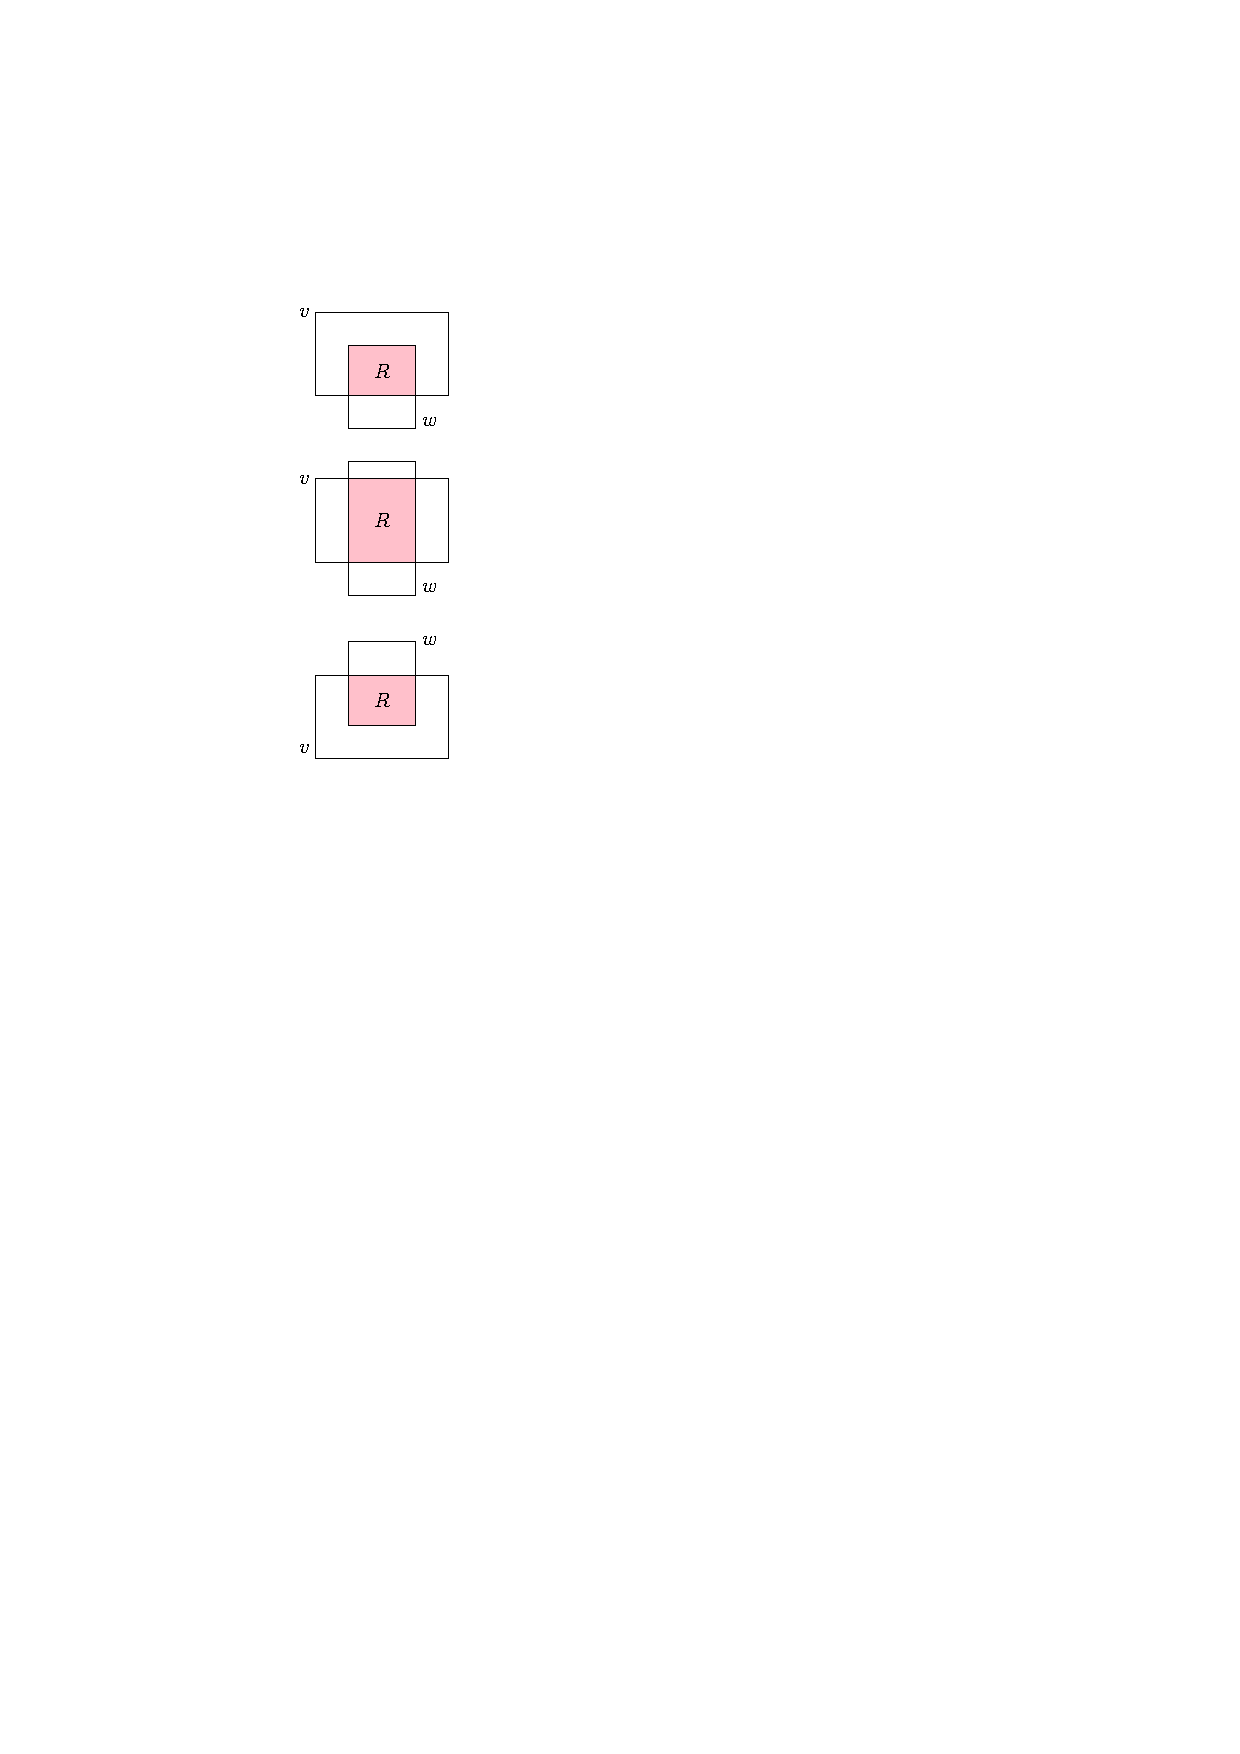
\includegraphics{figs/hvo-1} & 
   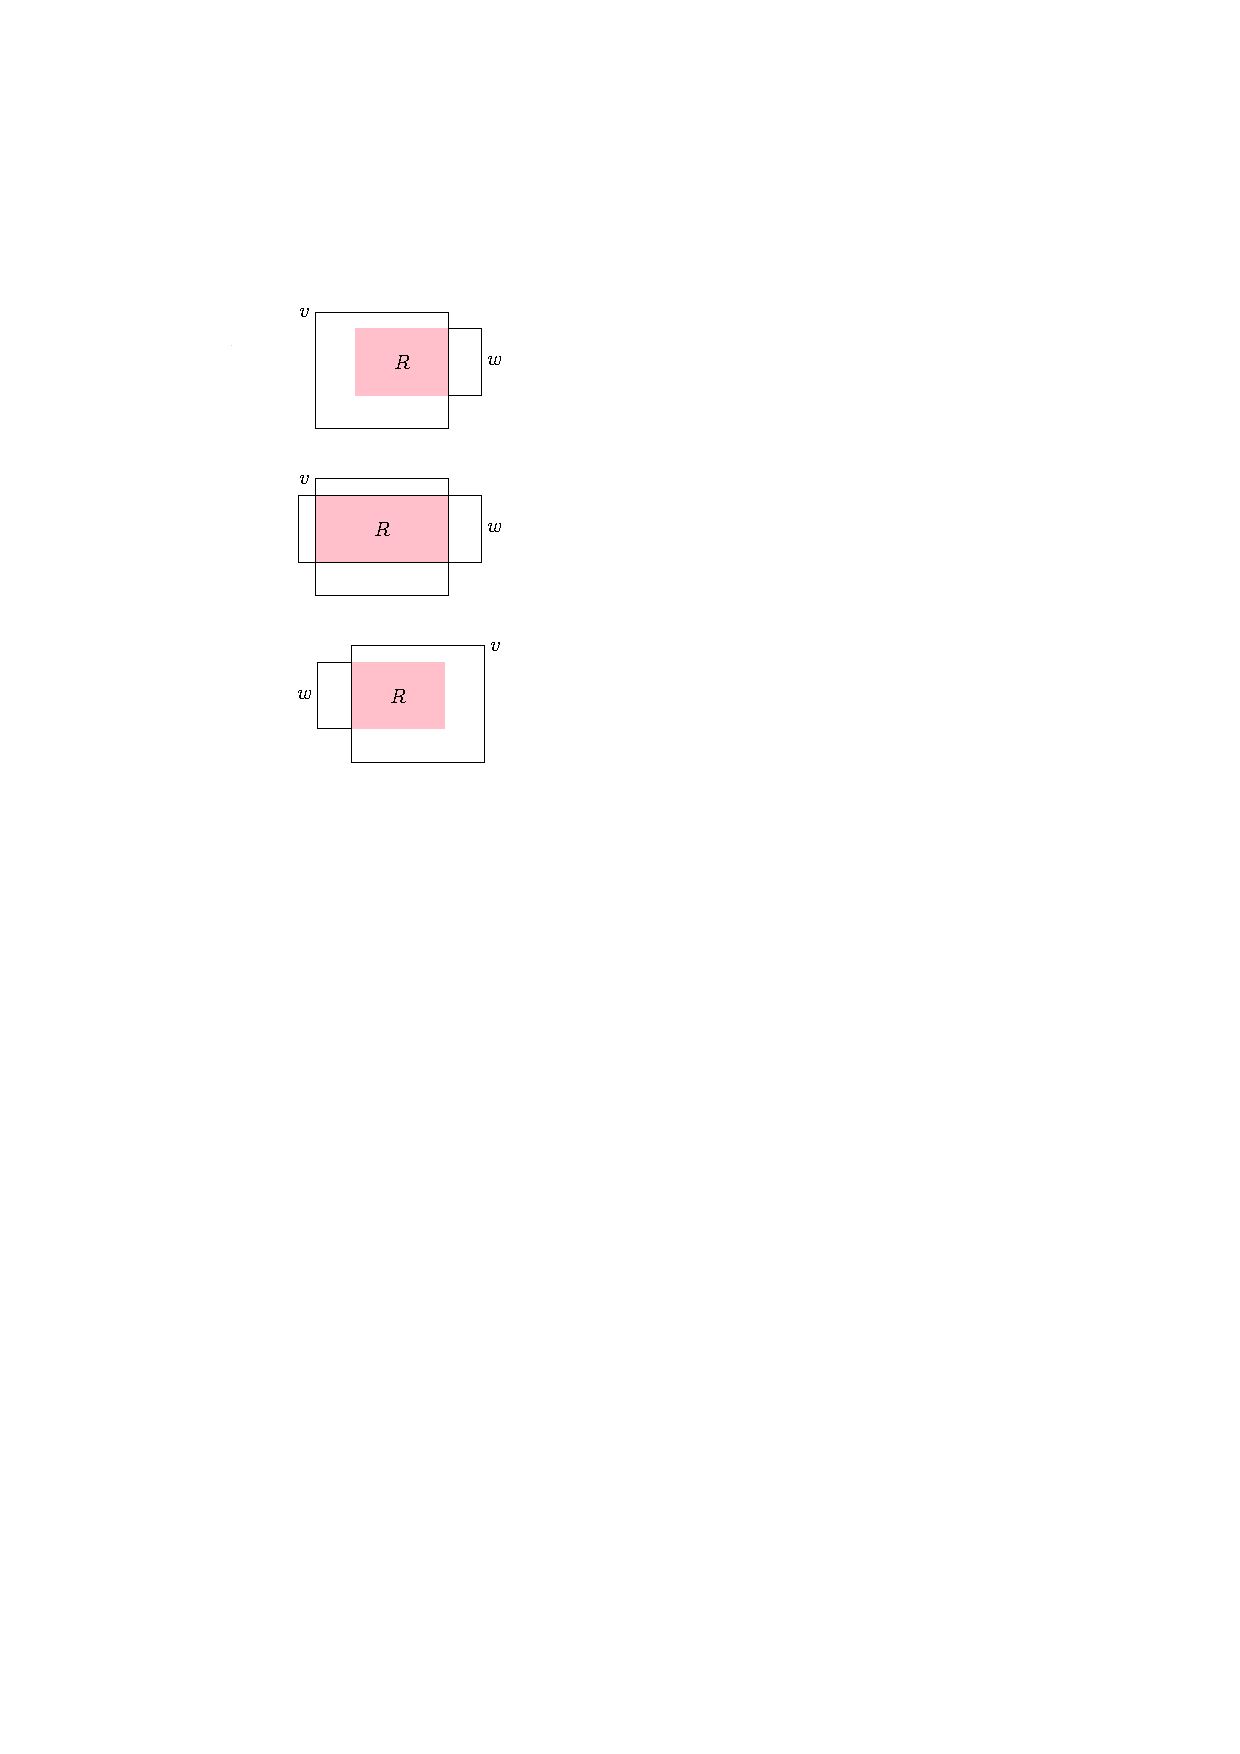
\includegraphics{figs/hvo-2} & 
   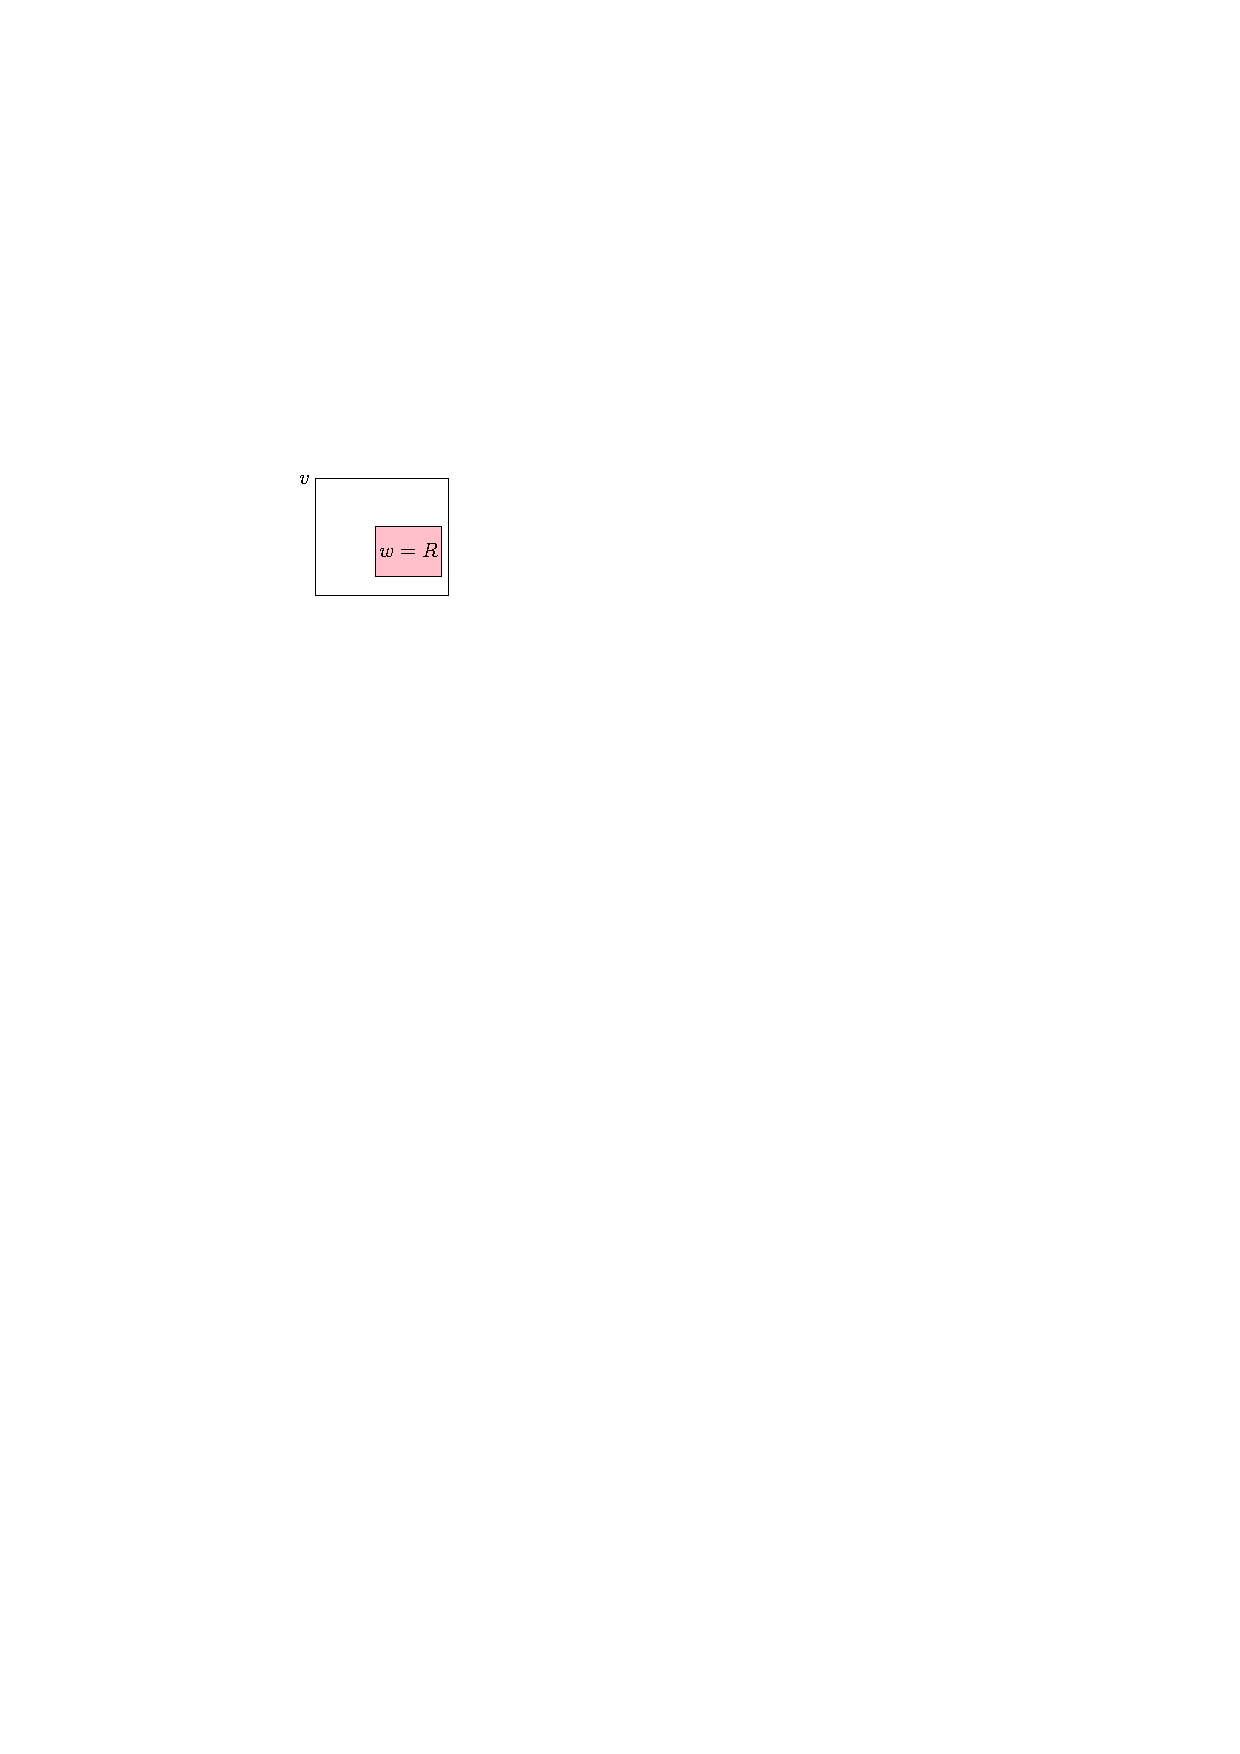
\includegraphics{figs/hvo-3} \\
   v-pairs & h-pairs & o-pair
   \end{tabular}
   \caption{Examples of v-pairs, h-pairs, and an o-pair.}
   \figlabel{hvo}
\end{figure}

Our proof works by finding a path in a rectangle intersection graph $G$
that defines a sequences of rectangles having properties that ensure
that these rectangles form a clique. See \figref{good-sequence} for an
illustration of the following definition:
\begin{dfn}\dfnlabel{hvo-alternating}
Let $v_1,\ldots,v_k$ be a sequence of rectangles and let
$R_i=\bigcap_{j=1}^i v_j$.  We say that $v_1,\ldots,v_k$ is
\emph{hvo-alternating} if
\begin{compactenum}
  \item for each $i\in\{2,\ldots,k\}$, $v_i\cap R_{i-1}\neq \emptyset$;
  \item for each $i\in\{2,\ldots,k\}$,
        $v_i$ does not contain any corner of $R_{i-1}$; and
  \item for each $i\in\{2,\ldots,k-1\}$, $(R_{i-1},v_i)$ and
        $(R_i,v_{i+1})$ are not both h-pairs and not both v-pairs.
\end{compactenum}
\end{dfn}

\begin{figure}
  \begin{center}
    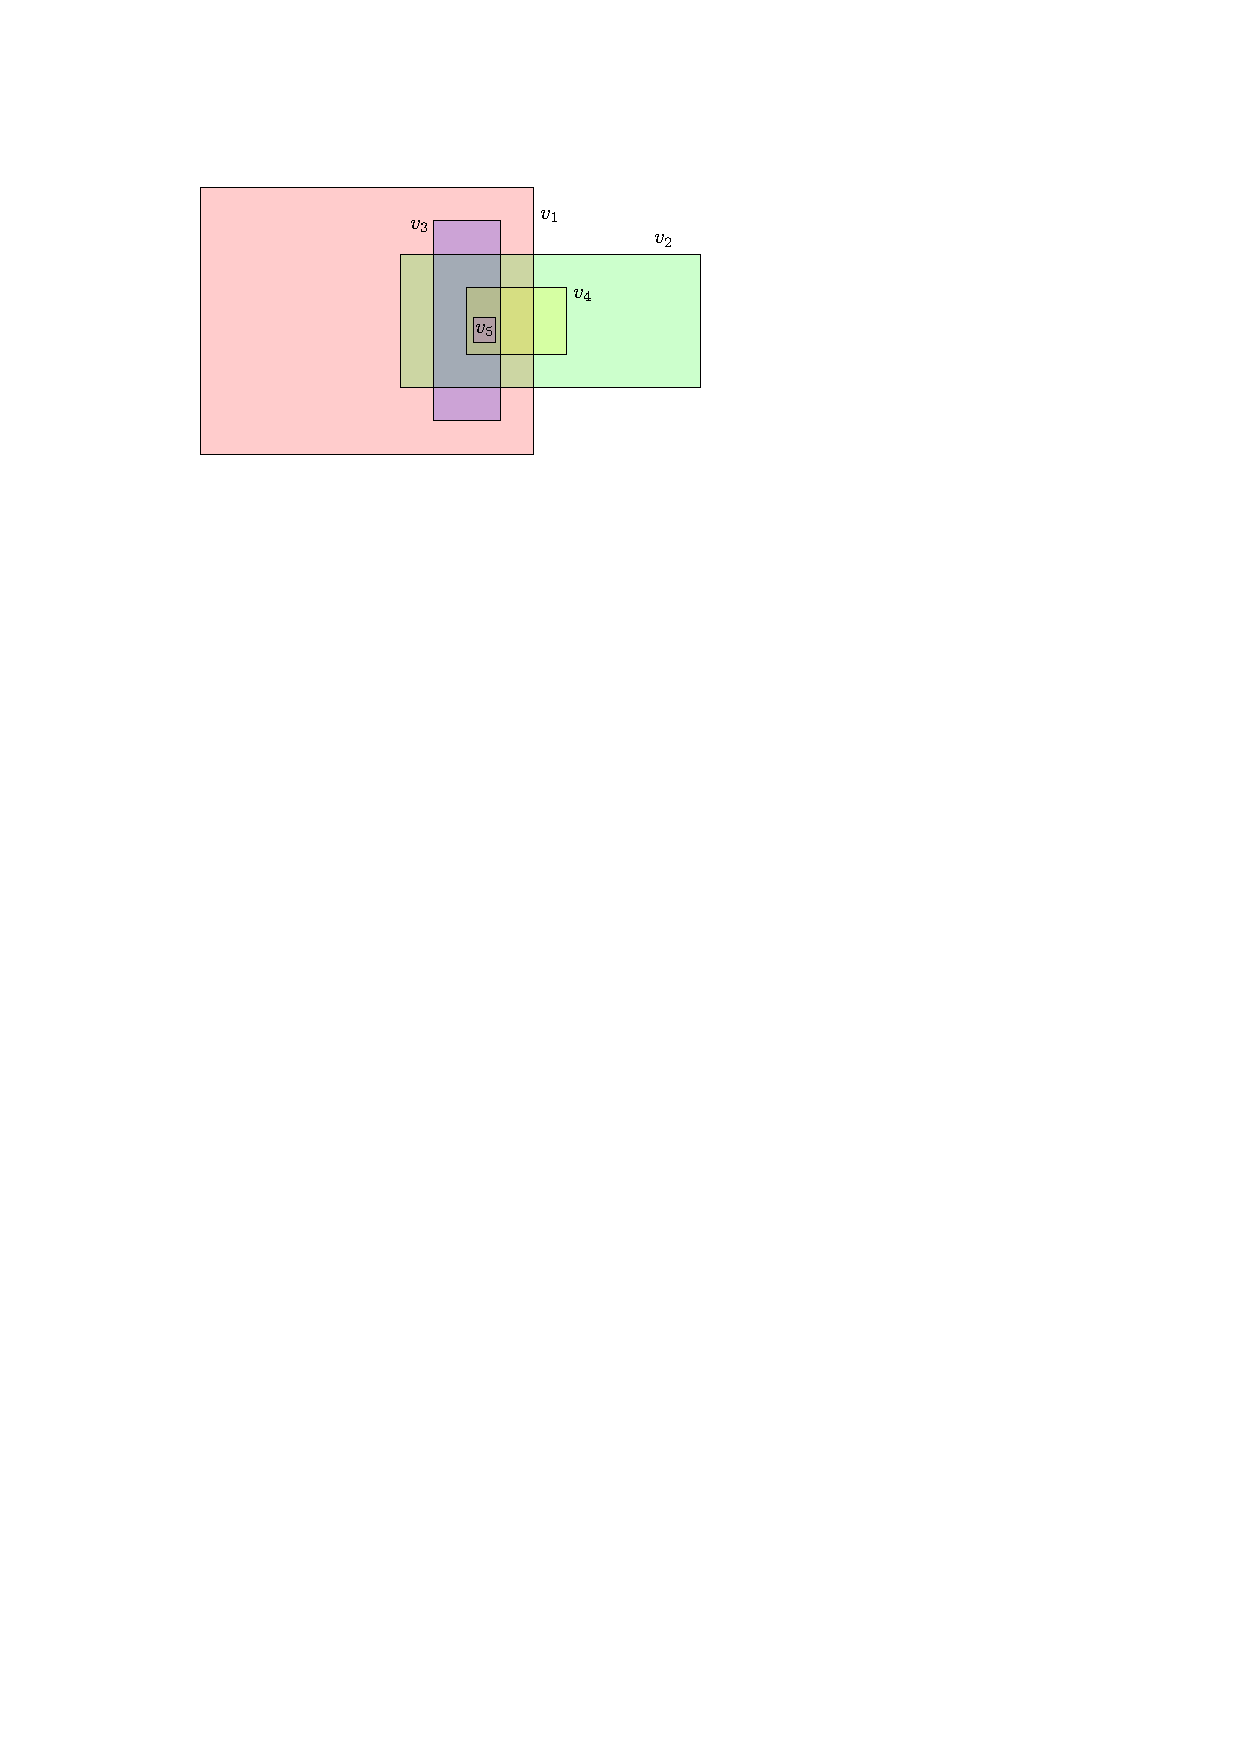
\includegraphics{figs/good-sequence}
  \end{center}
  \caption{An hvo-alternating sequence of rectangles.}
  \figlabel{good-sequence}
\end{figure}

Note that Property~1 in \dfnref{hvo-alternating}, with $i=k$ ensures that
$\bigcap_{j=1}^k v_i\neq\emptyset$.  If $v_1,\ldots,v_k$ are vertices in a
rectangle intersection graph $G$, then these vertices form a $k$-clique
in $G$.  Our proof works by attempting to grow an hvo-alternating
sequence, but sometimes this process stalls. The following lemma shows
that, when this process stalls, we can at least replace the last element
in the sequence.

%We will make use of the following simple geometric lemma:
%\begin{lem}\lemlabel{hv-triples}
%  If $v_1,v_2,v_3$ is an hvo-alternating sequence of rectangles then
%  $v_1\cap v_2\cap v_3=v_2\cap v_3$.
%\end{lem}
%
%\begin{proof}
%  Recall that, for any two sets $A$ and $B$, $A\supseteq B$ if and only
%  if $A\cap B = B$. Therefore, it is sufficient to show that $v_1\supseteq
%  v_2\cap v_3$.
%
%  If $(v_1,v_2)$ is an o-pair, then $v_1\supseteq v_2\supseteq v_2\cap
%  v_3$ and we are done.  Otherwise, assume without loss of generality
%  that $(R_1,v_2)=(v_1,v_2)$ is an h-pair, so that $(R_2,v_3)$ is not an
%  h-pair. Refer to \figref{geometric}.  In this case, $v_2\cap v_3$ is
%  contained in the rectangle $R^*$ whose top and bottom sides coincide
%  with those of $v_2$ and whose left and right sides coincide with
%  those of $v_1$. We finish by Observing that $v_1\supseteq R^*\supseteq
%  v_2\cap v_3$, as required.
%\end{proof}
%
%\begin{figure}
%  \begin{center}
%    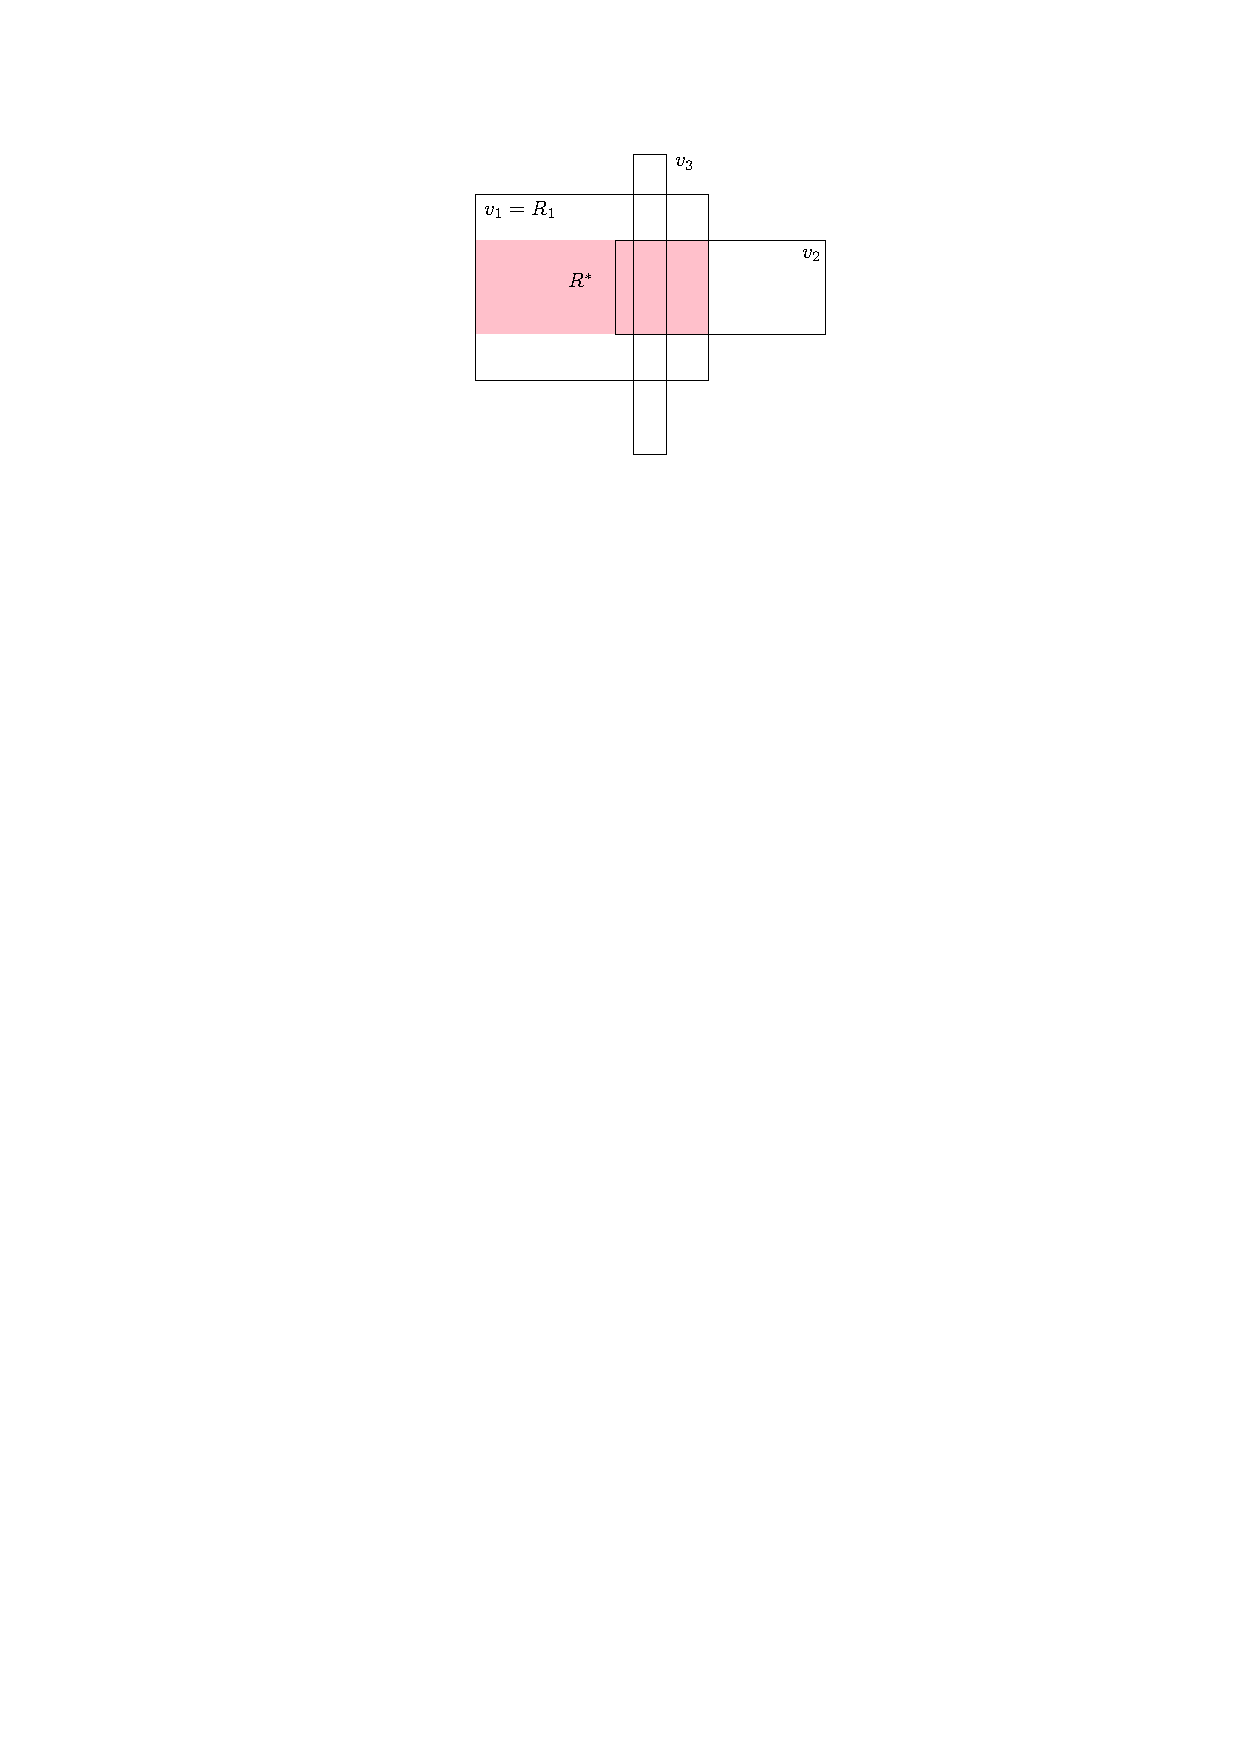
\includegraphics{figs/geometric}
%  \end{center}
%  \caption{The proof of \lemref{hv-triples}.}
%  \figlabel{geometric}
%\end{figure}
%
%Our proof attempts to grow an hvo-alternating sequence of rectangles
%$v_1,\ldots,v_k$. The following lemma shows that this entire sequence is,
%in some sense, represented by its last two elements.
%
%\begin{cor}\corlabel{hv-sequence}
%  If $v_1,\ldots,v_k$, $k\ge 2$, is an hvo-alternating sequence of
%  rectangles then $\bigcap_{i=1}^{k} v_i = v_{k-1}\cap v_k$.
%\end{cor}
%
%\begin{proof}
%  The case $k=2$ is trivial, so assume $k\ge 3$.
%  By \dfnref{hvo-alternating}, the three element sequence
%  $R_{k-2},v_{k-1},v_k$ is an hvo-alternating sequence so, by
%  \lemref{hv-triples},
%  \[  
%   \bigcap_{j=1}^k v_j = R_{k-2}\cap v_{k-1}\cap v_k = v_{k-1}\cap v_k
%   \enspace .  \qedhere 
%  \]
%\end{proof}

\begin{lem}\lemlabel{replacement}
  Let $v_1,\ldots,v_k$ be an hvo-alternating sequence of rectangles and
  define $R_i=\bigcap_{j=1}^i v_i$. Let $v$ be a rectangle such
  that 
  \begin{compactenum}
     \item $v\cap R_k\ne \emptyset$; 
     \item $v$ contains no corner of $R_k$; and 
     \item $v_1,\ldots,v_k,v$ is not hvo-alternating.
  \end{compactenum}
  Then $v_1,\ldots,v_{k-1},v$ is hvo-alternating.
\end{lem}

\begin{proof}
  Notice that $v_1,\ldots,v_k,v$ satisfies all the conditions to be
  hvo-alternating except that both $(R_{k-1},v_k)$ and $(R_k,v)$
  are both h-pairs or both v-pairs.  Without loss of generality assume
  that they are both h-pairs.

  It is sufficient to show that $(R_{k-1},v)$ is not a v-pair so that,
  by replacing $v_k$ with $v$ we are replacing the h-pair $(R_{k-1},v_k)$
  with a new with an h-pair or an o-pair.  But this is immediate, since
  $v$ intersects $R_k$ but does not intersect the top or bottom side
  of $R_k$.  Therefore $v$ cannot intersect the top or bottom side of
  $R_{k-1}\supseteq R_k$, so $(R_{k-1},v)$ is not a v-pair.
\end{proof}

A sequence $v_1,\ldots,v_k$ of rectangles is \emph{h-nesting} with
respect to a rectangle $R$ if, for each $i\in\{1,\ldots,k\}$, $(R,v_i)$
is an h-pair and, for each $i\in\{2,\ldots,k\}$, $(R\cap v_{i-1},v_i)$
is an h-pair.  See \figref{nesting}.  A \emph{v-nesting sequence} is
defined similarly by replacing h-pair with v-pair.

\begin{figure}
 \begin{center}
    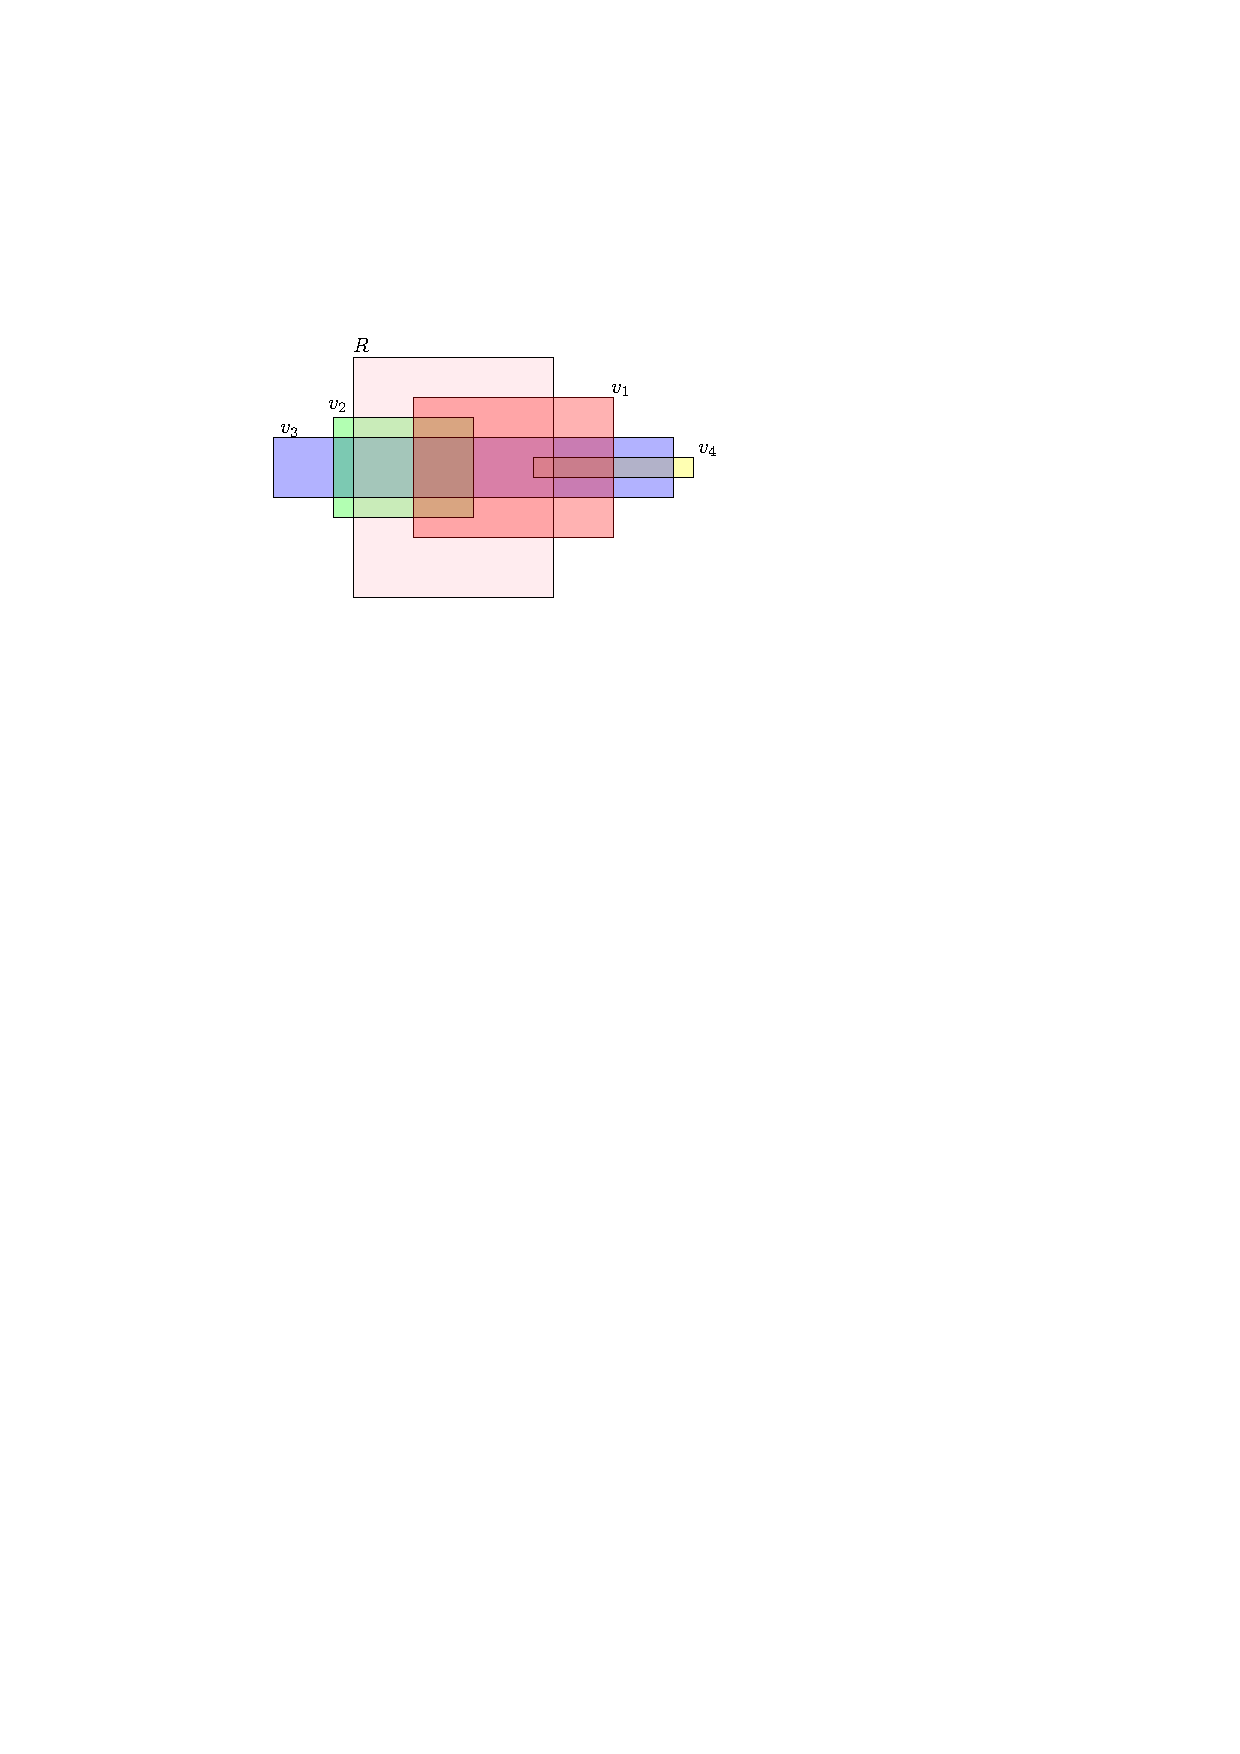
\includegraphics{figs/nesting}
 \end{center}
 \caption{Rectangles $v_1,\ldots,v_4$ that are h-nesting with respect to $R$.}
 \figlabel{nesting}
\end{figure}

\begin{lem}\lemlabel{nesting}
   If $v_1,\ldots,v_k$ is an h-nesting sequence or a v-nesting sequence
   with respect to $R$, then there exists a point $x\in R$ such that $|\{
   i: x\in v_i \}|\ge \lceil k/2\rceil$.
\end{lem}

\begin{proof}
   Assume, without loss of generality, that $v_1,\ldots,v_k$ is h-nesting
   sequence with respect to $R$.  Consider the sequence of horizontal
   strips $s_1,\ldots,s_k$, where each $s_i=(-\infty,\infty)\times
   (y_{i,1},y_{i,2})$ has top and bottom sides that coincide with those
   of $v_i$. Since, for each $i\in\{2,\ldots,k\}$, $(R\cap v_{i-1},v_i)$
   is an h-pair, $s_1\supseteq s_2\supseteq\cdots\supseteq s_k$.
   Let $\ell$ be a point on the left side of $R$ contained in $s_k$
   and let $r$ be a point on the right side of $R$ contained in $s_k$.
   Since $(R,v_i)$ is an h-pair, $v_i$ contains at least one of $\ell$
   or $r$, for each $i\in\{1,\ldots,k\}$.  Therefore, at least one of
   $\ell$ or $r$ is contained in at least $\lceil k/2\rceil$ rectangles
   in $v_1,\ldots,v_k$.
\end{proof}

\subsubsection{The Universal 2-Tree}

The \emph{height-$h$ $d$-branching universal 2-tree}, $T_{h,d}$ is
defined recursively as follows:
\begin{itemize}
  \item $T_{0,d}$ is a two-vertex graph with a single edge;
  \item For $h\ge 1$, $T_{h,d}$ is obtained from $T_{h-1,d}$ by adding,
     for each edge $vw \in E(T_{h-1,d})\setminus E(T_{h-2,d})$,
     $d$ new vertices $x_{1,vw}$ adjacent to both $v$ and $w$.
\end{itemize}
The \emph{root edge} of $T_{h,d}$ is the single edge of $T_{0,d}$.
The $i$-vertices of $T_{h,d}$ are the vertices in $V(T_{i,d})\setminus
V(T_{i-1,d})$ and the $i$ edges of $T_{h,d}$ are the edges in
$E(T_{i,d})\setminus E(T_{i-1,d})$.

Note that the number of $i$-edges in $T_{h,d}$ is given by the recurrence
\[
   m_i = \begin{cases}
           1 & \text{if $i=0$} \\
           2dm_{i-1} & \text{otherwise}
       \end{cases}
\]
which resolves to $(2d)^{i}$.  Thus, the total number of edges in
$T_{h,d}$ it not more than $(2d)^{h+1}$.

\section{The Result}

\begin{thm}\thmlabel{path-times-path}
  For each $k\in \N$, any rectangle intersection graph that contains
  $T_{4k-7,\iters}$ as a subgraph contains a clique of size $k$.
\end{thm}

\begin{proof}
  The cases $k=1$ and $k=2$ are trivial so, for the remainder of the proof
  we assume that $k\ge 2$.

  Let $G$ be a rectangle intersection graph that contains
  $T=T_{4k-7,\iters}$ as a subgraph.  We use the convention that
  $V(G)=V(T)$ so that vertices of $T$ are rectangles in $V(G)$.  If
  vertices $v$ and $w$ are adjacent in $T$, then $v\cap w \neq\emptyset$.

  We will attempt to define a path $v_1,\ldots,v_k$ in $T$ such that
  $v_1,\ldots,v_k$ is hvo-alternating. Since every hvo-alternating
  sequence has  non-empty intersection, this implies that $v_1,\ldots,v_k$
  form a clique in $G$.  The only cases in which we are unable to complete
  this path occur because some point $x\in\R^2$ is contained in a set $X$
  of $k$ vertices of $T$.  In these cases, the set $X$ forms a $k$-clique
  in $G$.

  Let $vw$ be the root edge of $T$. We set $v_1=v$ and use the convention
  that $v_0=w$.  We will perform $\iters$ iterations, each of which
  tries to add another vertex, $v_{i+1}$, to a partially constructed
  hvo-alternating path $v_1,\ldots,v_i$. During iteration $t$, for
  each $t\in\{1,\ldots,\iters\}$, the procedure will consider a
  level-$t$ vertex of $T$ to include in the path.  At the end of
  iteration $t$, the last vertex in the partially constructed sequence
  is always a level-$t$ vertex.

  At the beginning of iteration $t$, $v_i$ is a level-$(t-1)$ vertex, so
  $v_{i-1}$ and $v_i$ are both adjacent to a set $S$ of $4k-7$ level-$t$
  vertices.  Each of the rectangles in $S$ intersects $v_{i-1}$ and
  $v_i$ so, by \obsref{vidas-helly}, each rectangle in $S$ intersects
  $v_{i-1}\cap v_i$.  Therefore, by by \corref{alternating}, each of
  the rectangles in $S$ intersects $R_i=\bigcap_{j=1}^i v_j$.

  If each rectangle in $S$ contains a
  at least one corner of $R_i$, then some corner of $R_i$ is contained 
  in at least
  \[  \left\lceil |N_{i+1}(v_i)|/4]\right\rceil 
         = \left\lceil(4k-7)/4]\right\rceil = k-1
  \]
  rectangles.  Since these rectangles are open, there is a point $x$
  contained in these $k-1$ rectangles and in $v_{i}$.  The resulting set
  of $k$ rectangles therefore form a $k$-clique in $G$ and we are done.

  Otherwise, some rectangle $v\in S$ does not contain a corner of $R_i$.
  Notice that the sequence $v_1,\ldots,v_i,v$ is hvo-alternating except,
  possibly, that the pairs $(R_{i-1},v_i)$ and $(R_i,v)$ are both h-pairs
  or both v-pairs.  There are two cases to consider:
  \begin{enumerate}
     \item $v_1,\ldots,v_i,v$ is hvo-alternating. In this
       case we say that the procedure \emph{succeeds} in iteration $t$
       and we set $v_{i+1}=v$.

     \item $v_1,\ldots,v_i,v$ is not hvo-alternating.  In this case,
       we say that the procedure \emph{stalls} in iteration $t$.
       In this case, we \emph{change} $v_i$ by setting $v_i=v$. By
       \lemref{replacement} the resulting sequence is hvo-alternating,

       Note that in this case we have failed to make our path any
       longer. Instead, we have only replaced the last element with a
       level-$t$ vertex.  Regardless, the next iteration will try to
       extend the path with the new value of $v_i$.
  \end{enumerate}
  If we allow this procedure to run sufficiently long, then one of two
  cases occurs:
  \begin{enumerate}
     \item The procedure succeeds (Case~1, above) at least $k-1$ times.
     In this case, it finds $v_2,\ldots,v_k$, so that $v_1,\ldots,v_k$
     is an hvo-sequence whose vertices form a $k$-clique in $G$.

     \item During these $\iters$ iterations, some element of our sequence,
     $v_i$ takes on a sequence $S_i=v_{i,0},\ldots,v_{i,2(k-i)}$
     of $2(k-i)+1$ different values because the procedure stalls
     $2(k-i)$ times while trying to select $v_{i+1}$.  In this
     case, $S_i$ is either h-nesting or v-nesting with respect
     to $R_{i-1}$ so, by \lemref{nesting}, all the rectangles in
     $S_i$ have a point in common with $R_{i-1}$.  But $R_{i-1}$
     is the common intersection of $v_1,\ldots,v_{i-1}$.  Therefore
     $v_1,\ldots,v_{i-1},v_{i,0},\ldots,v_{i,k-i}$ all have a point in
     common and therefore form a $k$-clique in $G$.
  \end{enumerate}
  Therefore, the number of iterations required before this procedure finds
  a $k$-clique in $G$ is at most
  \[
      h = \sum_{i=2}^k (2(k-i)+1) = k + (k-2)(k+1) = k^2-2 \enspace .
  \]
  During these $h$ iterations, the procedure selects a level-$j$ vertex
  of $T$ for $j=1,2,\ldots,h$.  Since $T$ has height $k^2-2 = h$, the 
  procedure succeeds in finding a $k$-clique before running out of levels.
\end{proof}

\section{Discussion}

The problem we consider in this paper comes from trying to understand
which graphs have a decomposition into two path partitions whose bags
have bounded intersections.  This is turns out to be equivalent to the
more geometric problem of underdstanding which graphs are subgraphs of
rectangle intersection graphs of bounded clique size.  There are several
other ways we could generalize these problems:

\begin{op}
   A $d$-D box graph is a graph whose vertices are $d$-dimensional
   axis-aligned boxes.   What is the largest value of $r_d$ for which
   there exists a $k=k(r_d)$ such that, for every $r$-tree $T$ there is
   a $d$-D box graph $G=G(T)$ that contains $T$ as a subgraph and that
   does not contain any $k$-clique?
\end{op}

\thmref{path-times-path} shows that $r_2 < 2$, and the obvious
representation of trees (1-trees) as rectangle intersection graphs shows
that $r_2\ge 1$, so $r_2=1$.

For $d>2$, we can show that $r_d < 2d$ by using a universal $2d$-tree
along with the fact that the intersection of boxes is a box, and boxes
have only $2d$ sides.  The only lower-bound we know is $r_d>1$.  (What,
if anything, stops our proof from generalizing to $d$-D box graphs?)


Back in two dimension, if we let $C$ be a set of lines, we can consider
intersection graphs of \emph{$C$-oriented convex shapes}: convex bodies
whose boundaries consists of linear pieces, each of which is parallel to
some line in $C$.  (Axis-aligned rectangles are $C$-oriented where $C$
is the set consisting of the x-axis and y-axis.)

\begin{op}
   For a set $C$ of lines, let $\mathcal{G}_C$ denote the class of
   intersection graphs of $C$-oriented convex shapes.  Does there exist,
   for every finite line set $C$ and every $k\in N$, an $r=r(C)$ and
   an $r$-tree $T=T(C)$ such that every graph $G\in\mathcal{G}_C$ that
   contains $T$ as a subgraph contains a $k$-clique?
\end{op}

The techniques that we have used for axis-aligned rectangles and
boxes break down rather quickly.  For rectangle intersection graphs we
implicitly make use of the fact that if a $G$, has a 3-cycle $u,v,w$,
then the rectangles representing $u$, $v$, and $w$ have a point in common.
This is not true for intersection graphs of $C$-oriented convex
shapes, even when $|C|=3$.

\bibliography{op}
\bibliographystyle{plainurl}
\end{document}
